
\section{Uvod}
Algoritam majmuna \cite{ZHAOMA}  metaheuristički je optimizacijski algoritam utemeljen na načinu na koji se majmuni u prirodi penju na planine. Razvijen je za učinkovitu globalnu optimizaciju multimodalnih optimizacijskih problema  s kontinuiranim varijablama u visokim dimenzijama. 
\par
Funkcija cilja optimizacijskog problema može se zamisliti kao polje s planinama. Kako bi majmun pronašao najviši vrh u polju, izvodi 3 radnje:
\begin{enumerate}
	\item Penjanje 
	
	\item Gledanje i skakanje
	
	\item Salto
\end{enumerate}

Majmun se sa svoje početne točke penje uz planinu (Penjanje). U jednom trenutku staje, gleda oko sebe kako bi našao višu planinu i ako takva postoji, skače na nju (Gledanje i skakanje). Ponovno se penje uz planinu (Penjanje). Kako bi pronašli još višu planinu, mogu napraviti salto u novu domenu pretraživanja (Salto). Nakon što cijela populacija majmuna izvrši ovaj postupak dovoljno puta, dobije se izlaz algoritma koji je najviša točka koju su majmuni posjetili.

\par

U multimodalnim optimizacijskim problemima, broj lokalnih optimuma raste eksponencijalno s povećanjem dimenzije. Cilj salta u algoritmu je izbjegavanje prekomjernog lokalnog pretraživanja. Penjanje, koje ustvari je lokalno pretraživanje, koristi pseudogradijent koji se uvijek računa na temelju vrijednosti funkcije cilja za 2 točke (neovisno o dimenziji). To omogućava učinkovitiju optimizaciju u optimizacijskih problemima u visokim dimenzijama.

\section{Algoritam}
Algoritam prati opisani iterativni postupak penjanja majmuna dok se ne dosegne određeni broj iteracija $N$. Izlaz je položaj za koji je zabilježena najveća vrijednost funkcije cilja.

\begin{algorithm}
	\begin{algorithmic}[1]
		\Function{MA}{M, n, N, Nc, a, b, [c, d]}
		\State x = \Call{Postavljanje}{M, n}
		\State x* = x[0] 
		\For{iter = 1 to N}
		\State \Call{Penjanje}{Nc, x, x*, a}
		\State \Call{GledanjeSkakanje}{x, b}
		\State \Call{Penjanje}{Nc, x, x*, a}
		\State \Call{Salto}{x, [c, d]}
		\EndFor
		\State
		\Return x*
		\EndFunction
	\end{algorithmic}
	\caption{Algoritam majmuna}
\end{algorithm}



\subsection{Postavljanje početnih položaja}
Položaj majmuna predstavlja $n$-dimenzionalni vektor:
\begin{equation}
	\vec{x} = (x_1, x_2, \dots, x_n)
\end{equation}
Položaj $i$-tog od $M$ majmuna:
\begin{equation}
	\vec{x}_i = (x_{i1}, x_{i2}, \dots, x_{in})
\end{equation}

Na početku je potrebno postaviti početne položaje svih $M$ majmuna. Najjednostavnije je odrediti $n$-dimenzionalnu hiperkocku i iz nje uniformno uzorkovati položaj za svakog majmuna. Ako pojedini uzorkovani položaj ne zadovoljava ograničenja optimizacijskog problema, uzorkuje se ponovno dok ograničenja ne budu zadovoljena. Primjerice za hiperkocku $[0, 10]^{n}$:
\begin{algorithm}[H]
	\begin{algorithmic}[1]
		\Function{Postavljanje}{M, n}
		\State x = []
		\For{i = 1 to M}
		\Repeat
		\For{j = 1 to n}
		\State x[i][j] = rand(0, 10)
		\EndFor
		\Until{x[i] zadovoljava ograničenja}
		\EndFor
		\State
		\Return x
		\EndFunction
	\end{algorithmic}
	\caption{Postavljanje početnih položaja}
\end{algorithm} 

\subsection{Penjanje}
Cilj penjanja je doći do položaja za koji je funkcija cilja veća nego za trenutni. Za pomicanje koristi se pseudogradijent utemeljen na SPSA (\textit{simultaneous perturbation stochastic approximation}.)

\begin{enumerate}
	\item Za majmuna $i$ generira se vektor $\Delta\vec{x}_i = (\Delta\vec{x}_{i1}, \Delta\vec{x}_{i2}, \dots, \Delta\vec{x}_{in})$  gdje je
	\subitem  $\Delta\vec{x}_{ij} =
	\begin{cases}
		a & \text{s vjerojatnošću } 0.5 \\
		-a & \text{s vjerojatnošću } 0.5 \\
	\end{cases}$
	\subitem Parametar $a > 0$ zove se \textit{dužina koraka} i ovisi o optimizacijskom problemu.
	
	\item Računa se pseudogradijent funkcije cilja na položaju majmuna:
	\subitem $f'_i(\vec{x}_i) = (f'_{i1}(\vec{x}_i), f'_{i2}(\vec{x}_i), \dots, f'_{in}(\vec{x}_i))$ 
	
	\subitem $f'_{ij}(\vec{x}_i) = \frac{f(\vec{x}_i + \Delta\vec{x}_i) - f(\vec{x}_i - \Delta\vec{x}_i)}{2\Delta x_{ij}}$
	
	\item Neka je $\vec{y} = (y_1, y_2, \dots, y_n)$ gdje je
	\subitem $y_j = x_{ij} + a\cdot \text{sgn}(f'_{ij}(\vec{x}_i))$
	
	\item Ako $\vec{y}$ zadovoljava ograničenja, ažurira se položaj majmuna $\vec{x}_i \leftarrow \vec{y}$
\end{enumerate}

Za svakog majmuna se koraci 1 - 4 ponavljaju sve dok promjena funkcije cilja nije dovoljno mala ili dok se ne prođe maksimalan broj ponavljanja.

\begin{algorithm}[H]
	\begin{algorithmic}[1]
		\Function{Penjanje}{Nc, x, x*, a}
		\For{i = 1 to M}
		\Repeat
		\State $\Delta$x = []
		\State f' = []
		\State y = []
		\For{j = 1 to n}
		\State $\Delta$x[j] = rand([a, -a], [0.5, 0.5])
		\EndFor
		\For{j = 1 to n}
		\State f'[j] = (f(x[i] + $\Delta$x) - f(x[i] - $\Delta$x))/(2$\Delta$x[j])
		\EndFor
		\For{j = 1 to n}
		\State y[j] = x[i][j] + a*sgn(f'[j])
		\EndFor
		\If{y zadovoljava ograničenja} x[i] = y
		\EndIf
		\If{f(x[i]) > f(x*)} x* = x[i]
		\EndIf
		\Until{razlika f(x[i]) dovoljno mala ili dosegnut broj ponavljanja Nc}
		\EndFor
		\EndFunction
	\end{algorithmic}
	\caption{Penjanje}
\end{algorithm}



\subsection{Gledanje i skakanje}
Cilj gledanja i skakanja je prebaciti se na položaj u blizini čija je vrijednost funkcije cilja veća nego za trenutni. Definiran je parametar $b$ koji označava doseg majmunovog pogleda.

\begin{enumerate}
	\item Neka je $\vec{y} = (y_1, y_2, \dots, y_n)$ gdje je
	\subitem $y_j$ uzorkovan iz uniformne distribucije na $[x_{ij} - b, x_{ij} + b]$.
	
	\item Ako $\vec{y}$ zadovoljava ograničenja i vrijedi $f(\vec{y}) \ge f(\vec{x}_i)$, ažurira se položaj majmuna $\vec{x}_i \leftarrow \vec{y}$
\end{enumerate}

Za svakog majmuna se korak 1 ponavlja sve dok se ne zadovolji uvjet u koraku 2.

\begin{algorithm}[H]
	\begin{algorithmic}[1]
		\Function{GledanjeSkakanje}{x, b}
		\For{i = 1 to M}
		\Repeat
		\State y = []
		\For{j = 1 to n}
		\State y[j] = rand(x[i][j] - b, x[i][j] + b))
		\EndFor
		\Until{y zadovoljava ograničenja i f(y) >= f(x[i])}
		\State x[i] = y
		\EndFor
		\EndFunction
	\end{algorithmic}
	\caption{Gledanje i skakanje}
\end{algorithm}


\subsection{Salto}
Cilj salta je prebaciti se u novu domenu. Određuje se centroid položaja svih majmuna i svaki majmun radi salto u njegovom smjeru. Definiran je raspon $[c, d]$ iz kojeg se uniformno uzorkuje duljina salta.

Računa se centroid $p$:

\begin{equation}
	\vec{p} = \frac{1}{M} \sum_{i = 1}^{M} \vec{x}_i
\end{equation}

\begin{enumerate}
	
	\item Neka je $\vec{y} = \vec{x}_i + \alpha(\vec{p} - \vec{x}_i)$ gdje je
	\subitem $\alpha$ uzorkovan iz uniformne distribucije na $[c, d]$
	
	\item Ako $\vec{y}$ zadovoljava ograničenja, ažurira se položaj majmuna $\vec{x}_i \leftarrow \vec{y}$
\end{enumerate}

Za svakog majmuna se korak 1 ponavlja sve dok se ne zadovolji uvjet u koraku 2.

\begin{algorithm}[H]
	\begin{algorithmic}[1]
		\Function{Salto}{x, [c, d]}
		
		\State p = []
		
		\For{i = 1 to M}
		\State p += x[i]
		\EndFor
		
		\State p = p/M
		
		\For{i = 1 to M}
		\Repeat
		\State $\alpha$ = rand(c, d)
		\State y = x + $\alpha$ * (p - x[i])
		
		\Until{y zadovoljava ograničenja}
		\State x[i] = y
		\EndFor
		\EndFunction
	\end{algorithmic}
	\caption{Salto}
\end{algorithm}



\section{Programsko ostvarenje}
\subsection{Primjer funkcije za maksimizaciju}
Neka se maksimizira $n$-dimenzionalna funkcija:
\begin{align*}
	&f(\vec{x}) = -(\vec{x}^\intercal\vec{x}) \label{eq:fx} \tag{4.4} \\
	&\vec{x} \in [-100, 100]^n
\end{align*}
Funkcija ima maksimum u točki $\vec{0}$ i on iznosi $f(\vec{0}) = 0$. Minimum je na kutovima domene i iznosi $-100^2n$.

\begin{figure}[H]
	\centering
	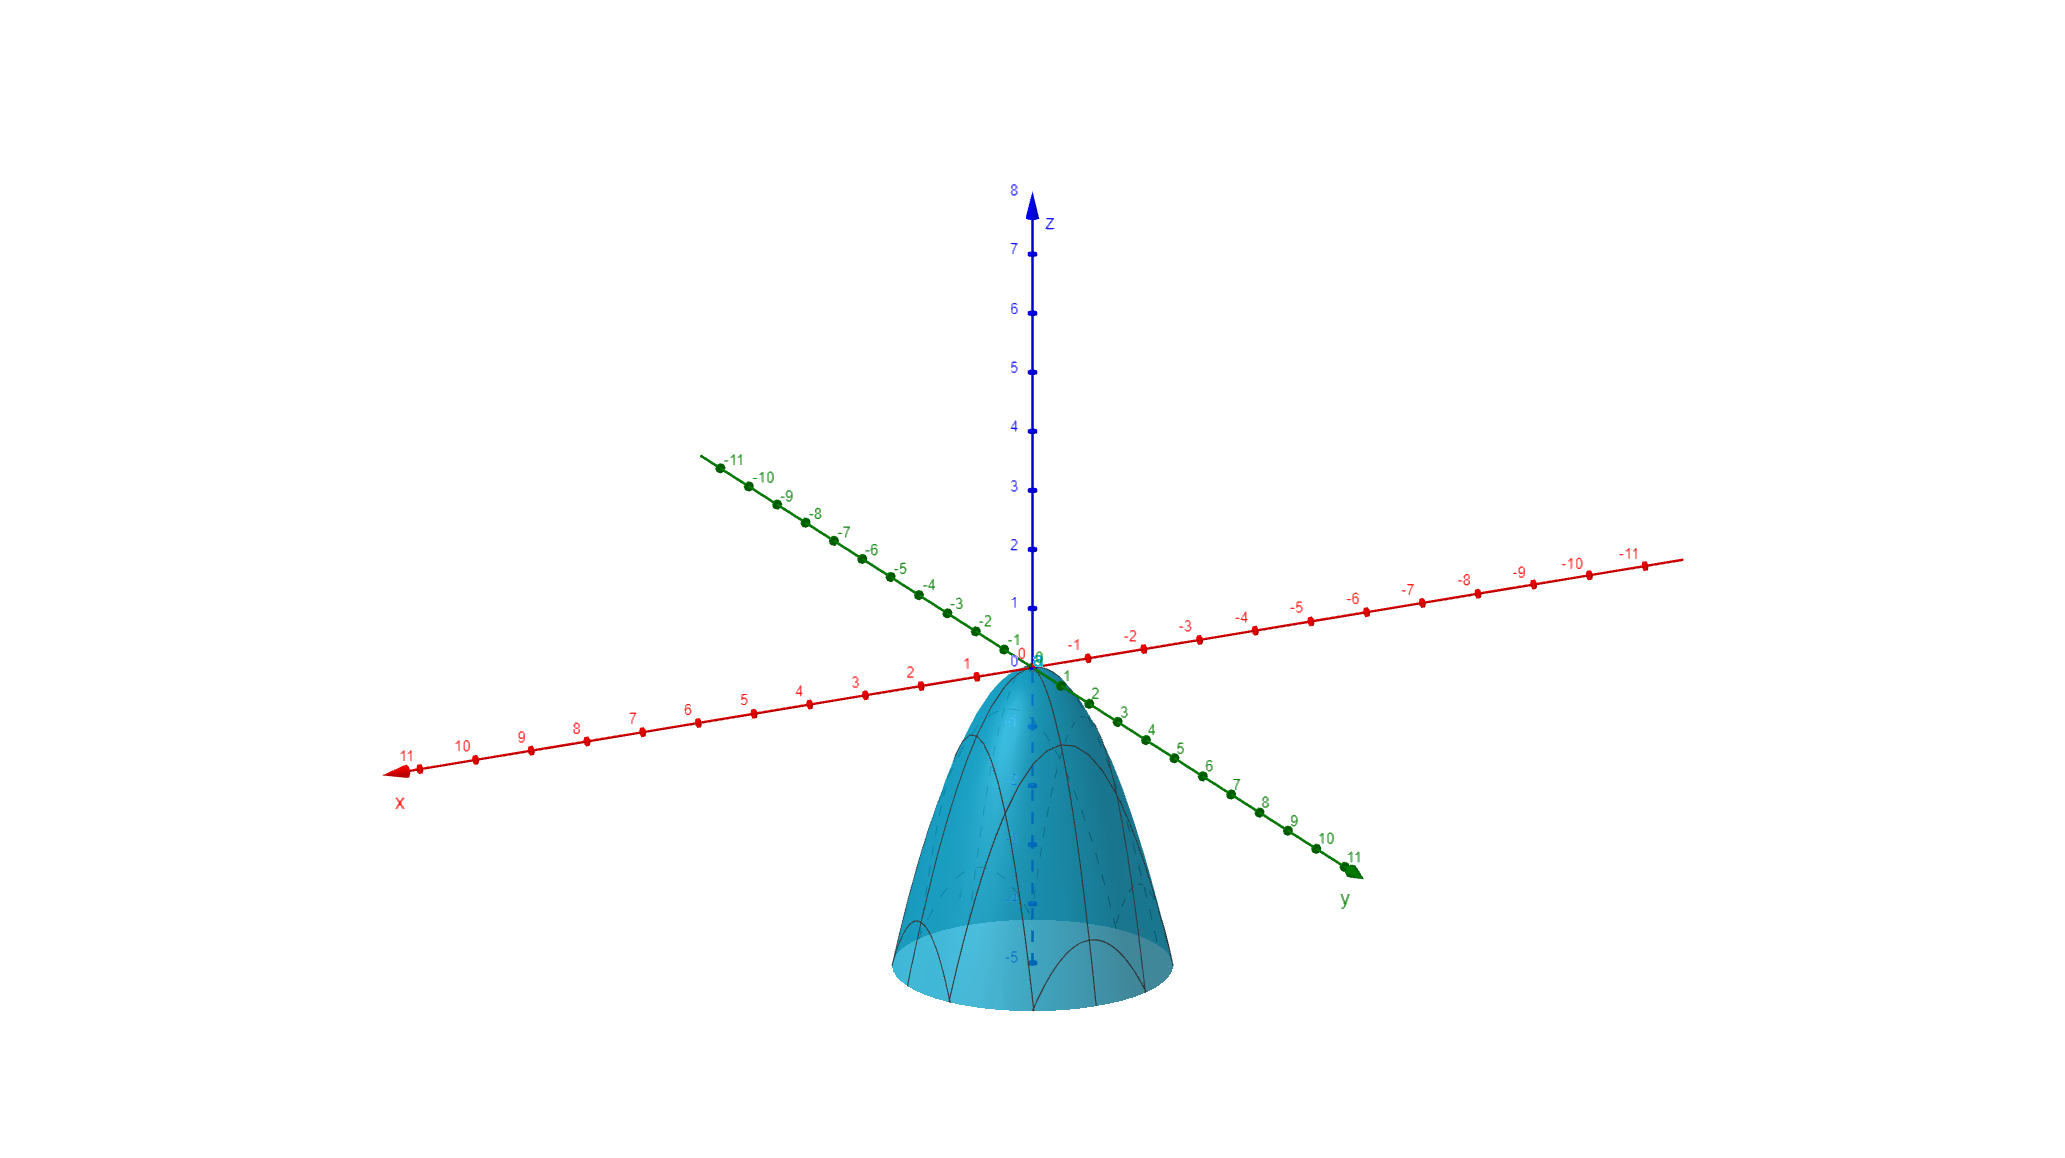
\includegraphics[width=14cm]{geogebra}
	\caption{Graf funkcije $f(\vec{x})$ za $n = 2$} 
	
\end{figure}

\subsection{Vlastito programsko ostvarenje}
Vlastito programsko ostvarenje algoritma majmuna povedeno je prevođenjem pseudokoda u programski jezik Python. Korištene su knjižnice programa za Python: \textit{numpy} i \textit{random}. Sastoji od klase \verb|MA| sa sljedećim metodama:

\begin{enumerate}
	\item \verb|__init__(self, M, N, Nc, a, b, c, d)|
	
	Instanciranje klase i postavljanje parametara algoritma
	
	
	\item \verb|optimize(self, f, cond, n, l, r)| 
	
	Optimizacija funkcije \verb|f| s funkcijom ograničenja \verb|cond|
	
	\item \verb|initialize(self, cond, l, r, M, n)| 
	
	Generiranje početnih položaja svih majmuna
	
	\item \verb|climb(self, M, Nc, n, X, a)| 
	
	
	\item \verb|watchJump(self, M, n, X, b)| 
	
	
	\item \verb|sumersault(self, M, n, X, c, d)| 
	
	
	\item Pomoćne funkcije:
	
	\subitem \verb|sampleHypercube(self, n, l, r)| 
	
	
	\subitem \verb|sampleWatch(self, n, x, b)| 
	
	\subitem \verb|sampleDx(self, n, a)| 
	
\end{enumerate}

\begin{tabular}{|m{1cm}|m{11cm}|}
	
	\hline
	\verb|M| & Broj majmuna \\
	\hline
	\verb|N| & Broj iteracija algoritma \\
	\hline
	\verb|Nc| & Broj skakanja \\
	\hline
	\verb|f| & Funkcija koja se optimira \\
	\hline
	\verb|cond| & Funkcija kojom se provjerava zadovoljenost ograničenja \\
	\hline
	\verb|n| & Dimenzionalnost ulaza funkcije \\
	\hline
	\verb|a| & Duljina skoka \\
	\hline
	\verb|b| & Udaljenost pogleda \\
	\hline
	\verb|c| & Donja granica duljine salta \\
	\hline
	\verb|d| & Gornja granica duljine salta \\
	\hline
	\verb|l| & Donja granica u svakoj dimenziji hiperkocke  \\
	\hline
	\verb|r| & Donja granica u svakoj dimenziji hiperkocke \\
	\hline
	\verb|X| & Lista svih majmuna \\
	\hline
	\verb|x| & Položaj pojedinog majmuna \\
	\hline
\end{tabular}


Na primjer, optimira se funkcija \eqref{eq:fx} s $n = 30$ dimenzija koristeći $M = 5$ majmuna, $N = 60$ iteracija, $Nc = 500$ skokova, duljinom koraka $a = 0.0001$, udaljenošću pogleda $b = 10$ i duljinom salta $[c, d] = [-1, 1]$.

Klasa \verb|MA| nalazi se u datoteci \verb|ma.py|. Može se pokrenuti na sljedeći način:


\begin{framed}
	\begin{verbatim}import ma
		import numpy as np
		import matplotlib.pyplot as plt
		
		f = lambda x : -np.dot(x, x)
		cond=lambda x : np.max(x) < 100 and np.min(x) > -100
		
		m = ma.MA(M=5, N=60, Nc=500, a=0.0001, b=10, c=-1, d=1)
		x, fs = m.optimize(f=f, cond=cond, n=30, l=-100, r=100)
		
		print("x* =", x)
		print("f(x*) =", f(x))
		
		plt.plot(range(1, len(fs)), fs[1:])
		plt.show()
	\end{verbatim}
\end{framed}

\noindent Izlaz ovog primjera je:
\begin{framed}
	\begin{verbatim}
		x* = [ 3.29615006  4.05143309  ...  -3.15835887]
		f(x*) = -330.1389091136464
	\end{verbatim}
\end{framed}

\begin{figure}[h]
	\centering
	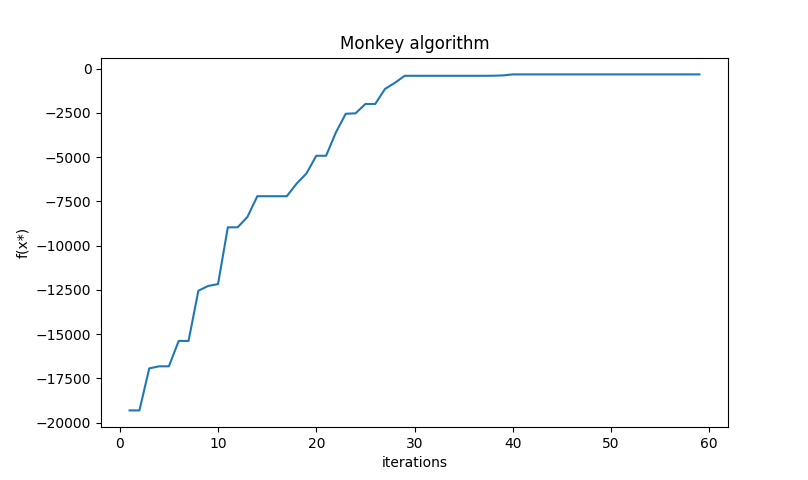
\includegraphics[width=14cm]{Figure_1}
	\caption{Graf ovisnosti izlaza funkcije o broju iteracija za dani primjer} 
	
\end{figure}



\subsection{Programsko ostvarenje MQL5}
\label{sec:mql5majmun}
Programsko ostvarenje algoritma majmuna autora A. Dika\cite{DIKMA} može se preuzeti na internetskoj stranici \href{https://www.mql5.com/en/articles/12212}{MQL5}. Važno je napomenuti da se ovo ostvarenje razlikuje se od onog u pseudokodu u pogledu funkcija \textit{gledanje i skakanje} i \textit{salto}.

Za pokretanje potrebno je instalirati program \href{https://www.metatrader5.com/en}{Meta Trader 5}, otvoriti korisnički račun i unutar programa otvoriti dijagram za proizvoljni \textit{symbol}. Zip dokument s algoritmima smjesti se u podatkovnu strukturu programa MQL5.


 Za pokretanje algoritma na preddefiniranim testnim funkcijama odabire se \verb|Scripts/Test_OA_MA.mq5| u \textit{Navigatoru}. U novootvorenom prozoru postavljaju se parametri i pokreće se algoritam koji u stvarnom vremenu prikazuje položaje majmuna na hiperravnini i ispisuje rezultat i pogrešku. 

\begin{figure}[H]
	\centering
	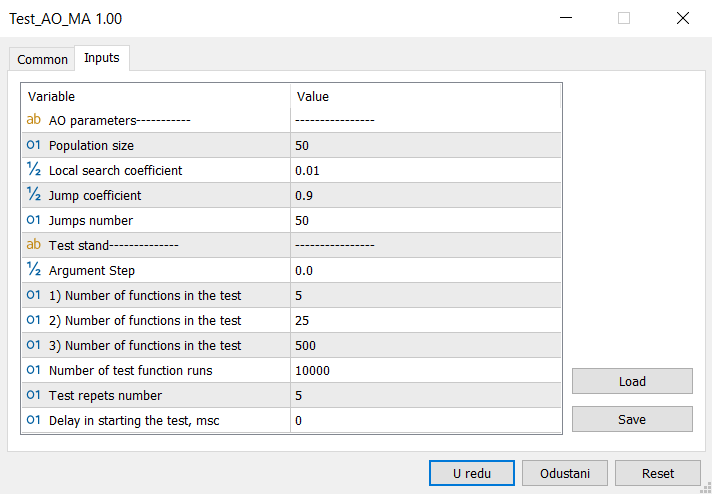
\includegraphics[width=14cm]{mt51}
	\caption{Odabir parametara algoritma u Meta Traderu 5} 
	
\end{figure}

\begin{figure}[H]
	\centering
	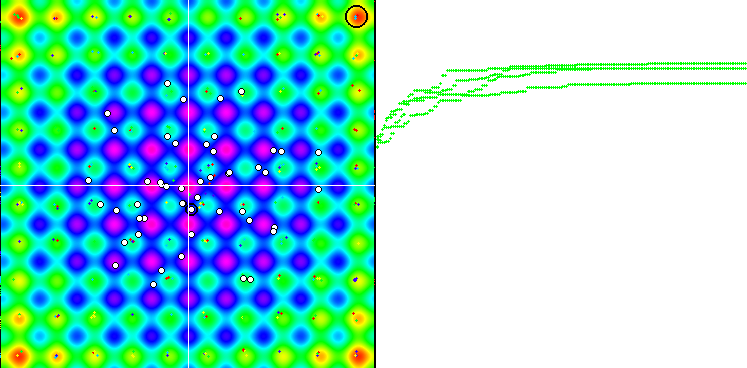
\includegraphics[width=14cm]{mt52}
	\caption{Položaji majmuna (bijele točke) u stvarnom vremenu na hiperravnini (lijevo) i izlazi funkcije cilja za 4 pokretanja algoritma (desno)}
	\centering
	
\end{figure}

\noindent Ispis je:
\begin{framed}
	\begin{verbatim}
		5 Rastrigin's; Func runs 10000 result: 68.03668259
		Score: 0.84301
		25 Rastrigin's; Func runs 10000 result: 55.4356683739
		Score: 0.68688
		500 Rastrigin's; Func runs 10000 result: 41.238597562
		Score: 0.51097
		=============================
		5 Forest's; Func runs 10000 result: 0.445023241351
		Score: 0.25173
		25 Forest's; Func runs 10000 result: 0.183789574445
		Score: 0.10396
		500 Forest's; Func runs 10000 result: 0.062930759789
		Score: 0.03560
		=============================
		5 Megacity's; Func runs 10000 result: 2.63999999999
		Score: 0.22000
		25 Megacity's; Func runs 10000 result: 1.11199999999
		Score: 0.09267
		500 Megacity's; Func runs 10000 result: 0.3276
		Score: 0.02730
	\end{verbatim}
\end{framed}

Vlastite funkcije za optimizaciju definiraju se u \verb|Include/Math/functions.mqh| u programskom jeziku temeljenom na C++. Funkcija \eqref{eq:fx} može se definirati na sljedeći način:

\begin{framed}
	\begin{verbatim}
		class C_Sphere : public C_Function
		{
			public: //====================================
			C_Sphere ()
			{
				SetNamFun ("Sphere");
				
				SetMinX (-100.0);
				SetMaxX ( 100.0);
				SetMinY (-100.0);
				SetMaxY ( 100.0);
				
				SetMinFun   (-20000.0);       //4 points
				SetMinFuncX (100.0);
				SetMinFuncY (100.0);
				
				SetMaxFun   (0.0);           //1 points
				SetMaxFuncX (0.0);
				SetMaxFuncY (0.0);
			}
			
			private: //===================================
			double Core (double x, double y)
			{
				double res = -(x*x + y*y);
				return(res);
			}
		};
	\end{verbatim}
\end{framed}

Za pokretanje optimizacije proizvoljne funkcije, potrebno je u \verb|Test_OA_MA.mq5| u funkciji \verb|void OnStart()| upisati poziv funkcije \verb|FuncTests|. Parametri funkcije su: funkcija, dimenzija $n/2$ i boja linije na grafu funkcije cilja. Primjerice za funkciju \verb|C_Sphere|:

\begin{framed}
	\begin{verbatim}
		C_Sphere F;
		FuncTests(F, 15, clrLime);
	\end{verbatim}
\end{framed}


Optimira se funkcija \eqref{eq:fx} s  $n = 30$ dimenzija s $M = 50$ majmuna, $N = 50000$ iteracija, $Nc = 50$ skokova, duljinom koraka $a = 0.01$ i udaljenošću pogleda $b = 0.9$.


\begin{figure}[H]
	\centering
	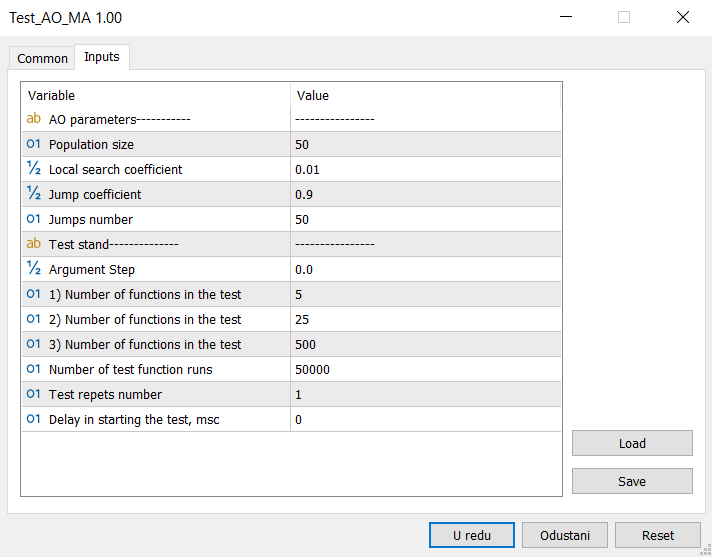
\includegraphics[width=14cm]{mt53}
	\caption{Odabir parametara algoritma za primjer}
	\centering
\end{figure}

\begin{figure}[H]
	\centering
	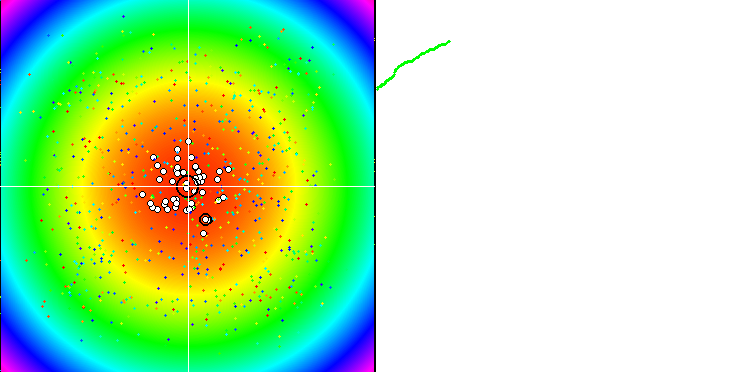
\includegraphics[width=14cm]{mt54}
	\caption{Položaji majmuna na hiperravnini i izlazi funkcije cilja tijekom izvođenja}
	\centering
\end{figure}

\begin{figure}[H]
	\centering
	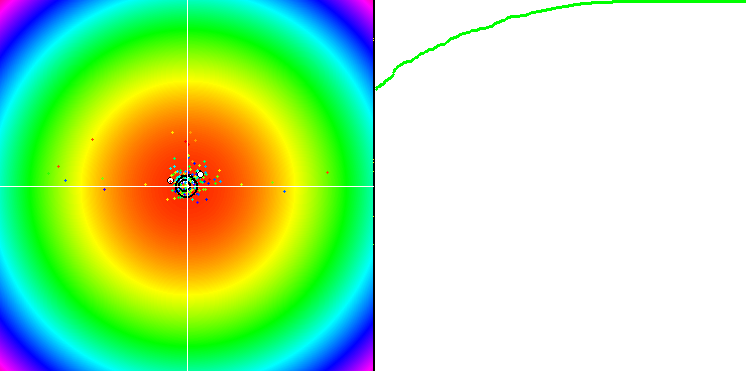
\includegraphics[width=14cm]{mt55}
	\caption{Položaji majmuna na hiperravnini i izlazi funkcije cilja nakon izvođenja}
	\centering
\end{figure}

\noindent Ispis je:
\begin{framed}
	\begin{verbatim}
		15 Sphere's; Func runs 50000 result: -2.5525976674831137
		Score: 0.99987
	\end{verbatim}
\end{framed}








\section{Primjene}

\subsection{Optimizacija hibridnih mikromreža}
Izmijenjeni algoritam majmuna upotrebljen je za optimizaciju konfiguracije komponenti hibridnih mikromreža.\cite{ITUARTEVILLARREAL2012344} Minimizirana je cijena i emisija stakleničkih plinova. Algoritam je izmijenjen uvođenjem meteoroloških faktora.


\subsection{Grupiranje}
Hibridni algoritam majmuna utemeljen na operatoru pretraživanja iz algoritma kolonije pčela upotrebljen je za grupiranje. \cite{Chen2014} Pokazano je da ima dobre performanse na sintetičkim i stvarnim skupovima podataka.

\subsection{0-1 problem naprtnjače}
Izmijenjenim algoritam majmuna predložen je za rješavanje 0-1 problema naprtnjače.\cite{ZHOU2016817} Lokalno pretraživanje ojačano je pohlepnima algoritmom a salto je izmijenjen kako bi se izbjeglo upadanje u lokalne optimume. Uveden je i kooperativni proces radi ubrzanje konvergencije. Pokazano je da je izmijenjeni algoritam majmuna učinkovita alternativa za rješavanje ovog problema.

\subsection{Raspoređivanje zadataka u računarstvu u oblaku}
Algoritam majmuna primijenjen je na raspoređivanje zadataka u računarstvu u oblaku.\cite{8313789} Minimizirana je cijena i maksimizirana iskorištenost kako bi se pružila bolja usluga klijentu. Pokazano je da takav algoritam radi učinkovitije od prethodno predloženih.

\subsection{Flow-shop scheduling}
Za NP-teški kombinatorni problem \textit{flow-shop scheduling} upotrebljen je hibridni algoritam majmuna s pod-populacijama.\cite{MARICHELVAM201782} Algoritam majmuna nadmašio je mnoge heurističke i metaheurističke algoritme iz literature.

\subsection{Raspoređivanje elektroničkih komponenata u računalima}
Algoritam majmuna korišten je za optimiziranje problema raspoređivanja elektroničkih komponenata u računalima.\cite{Kuliev_2018} Pokazano je da daje učinkovitija rješenja nego genetski algoritam.

\subsection{Set cover problem}
Za rješavanje \textit{set cover} problema, dizajniran je binarni algoritam majmuna.\cite{Crawford2020} Izmijenjen je proces penjanja majmuna i dodan je proces kooperacije. Pokazuje se da takav algoritam nadmašuje mnoge heurističke i metaheurističke algoritme iz literature. 


\subsection{Prepoznavanje tumora u MRI slikama mozga}
Automatizirani algoritam majmuna korišten je pronalaženje i segmentaciju lokacija tumora na MRI slikama mozga.\cite{Alagarsamy_2020} Tehniku je moguće upotrijebiti za pomoć radiolozima pri pronalaženju tumora.
